%% This is an example first chapter.  You should put chapter/appendix that you
%% write into a separate file, and add a line \include{yourfilename} to
%% main.tex, where `yourfilename.tex' is the name of the chapter/appendix file.
%% You can process specific files by typing their names in at the 
%% \files=
%% prompt when you run the file main.tex through LaTeX.
\chapter{Feature Selection for Classification}

Feature selection can be found in many areas of data mining and machine learning, such as classification, clustering, association rules, and regression. We focus on classification problem as the machine learning model. Feature selection algorithms aims to produce a subset of features that could improve the performance of the classifier that follows the feature selection process. In case of classifier that is used for prediction problem, feature selection could provide faster and more cost-effective predictors.

A paper by Liu \cite{Liu:2005} described the feature selection process in a simple way, that it firstly selects a subset of original features, then measures the optimality of a subset by using certain evaluation criterion. The challenge of the feature selection process lies on finding an optimal feature subset, which usually is intractable (hard to control) and some problems are even NP-Hard problems. With that, it is even more challenging to apply feature selection on high-dimensional data or big data. A common approach to easily conquer big data problems is to use parallel processing. Recent study by Singh \cite{Singh:2009} proposed a parallel approach to handle large scale feature selection specific for logistic regression problem. Several other parallel feature selection approaches also exist. However, the study over the advantages and drawbacks of those algorithms are still limited.

This chapter explains the categories of feature selection method in Section \ref{ch2:catg} and key steps or characteristics of feature selection in Section \ref{ch2:step}. Then, we list down several existing feature selection algorithms. Then we describe those algorithms that represents characteristics of different approaches in Section \ref{ch2:alg}. We discovered some feature selection algorithms that have been applied or proposed using parallel processing. In Section \ref{ch2:par}, those particular algorithms are explained. Finally in Section \ref{ch2:sel}, we choose an algorithm that we implement in the next chapter and we explain the reason for choosing it.

\section{Feature Selection Categories}\label{ch2:catg}

Feature selection algorithms can be categorized based on its evaluation criteria into three categories: 

\begin{enumerate}
\item \textbf{Filter methods}
\newline Filter methods apply statistical measures to assign a scoring to each feature and then decide to remove or not the respective features. These methods often consider each feature independently or with regard to the dependent variable. Commonly used filter methods are Chi-square test, information gain and correlation coefficient scores. 
\newline Filter methods rely on general characteristics of the data to evaluate and select feature subsets without involving any mining algorithm. Filter methods use a suitable criterion to score the features. One approach is: feature are then ranked or ordered based on the evaluation score. This approach is known as variable ranking. A threshold is then used to remove features having evaluation score below the threshold. This can be seen as to filter out less relevant features before classification. Another approach is to firstly generate all possible subsets and evaluate the score to determine whether the it is a subset that contains only relevant features. A feature is considered relevant when it has useful information about the different classes in the data. This property can be defined as feature relevance, which provides a measurement of the feature’s usefulness in discriminating the different classes \cite{Chandrashekar:2014}.

\item \textbf{Wrapper methods}
\newline Wrapper methods, like feature elimination algorithm, prepare different combinations of set of features, evaluate them using a prediction model, assign a score based on model accuracy and compare with other models. This method considers the selection of a set of features as a search problem, which can use best-first search as a methodical algorithm, random hill-climbing algorithm as a stochastic algorithm, forward/backward passes as a heuristic algorithm, or any other search methods. 
\newline Wrapper methods requires a predetermined mining algorithm or a predictor as a black box and uses its performance as the criterion to evaluate subsets. Since evaluating $2^N$ subsets becomes a NP-hard problem, suboptimal subsets are found by employing search algorithms, which find a subset heuristically. 

\item \textbf{Embedded methods}
\newline This model attempts to take advantage of the filter and wrapper models by exploiting their different evaluation criteria in different search stages.
\newline Embedded methods learn which features best contribute to the accuracy of the model while the model is being created. Commonly used embedded methods are LASSO (which selects a few sparse features), ElasticNet, and Ridge Regression.
\end{enumerate}


\section{Key Steps of Feature Selection}\label{ch2:step}

Liu's work in \cite{Liu:2005} summarizes the four basic steps in feature selection process, as depicted in Figure \ref{fig:img1}. Subset generation step produces candidate feature subsets for evaluation. Each candidate subset is evaluated and compared with the previous best one according to a certain evaluation criterion. If the new subset is better, it replaces the previous best subset. The process of subset generation and evaluation is repeated until a given stopping criterion is satisfied. The selected best subset usually needs to be validated by prior knowledge or different tests. The detail of the four key steps are explained below.

\begin{figure}[tb]
	\centering
	\includegraphics[scale=0.75]{img/img1}
	\caption{Four steps of feature selection (Source: \cite{Liu:2005})} \label{fig:img1}
\end{figure}

\begin{enumerate}
	\item \textbf{Subset generation}
	\newline It is a search problem that can be seen as a heuristic search, which produces candidate feature subsets for evaluation. Each state in the search space specifies a candidate subset for subset evaluation. The quality of searching depends on two basic issues.
	\newline First, search starting point determines the search direction. Forward selection starts from an empty set and incrementally add features. Backward selection starts with a full set and incrementally remove features. Bi-directional selection starts with both ends and add and remove features simultaneously. The quality of the subset produced on those search strategies heavily depends on the order of the features in the subset. In the case of getting trapped in the local minima, the subset is no longer the most optimal subset. Random selection tries to avoid that by starting with randomly selected subset \cite{Doak:1992}.
	\newline Second, search strategy could affect the processing time. A data set with $k$ features has $2^k$ candidate subsets. Thus, the search space is exponential and could become not scalable for large number of $k$. Different search strategies have been explored: complete, sequential, and random search.
	
	\begin{itemize}
	\item \textbf{Complete search} guarantees to find the optimal result. It does not have to be exhaustive. Different heuristic functions can reduce the search space without jeopardizing the chances of finding the optimal result. Hence, although the search space is $O(2^N)$, a smaller number of subsets are evaluated.
	\item \textbf{Sequential search} gives up completeness and thus risks losing optimal subsets. There are many variations to the greedy hill-climbing approach, such as \textit{sequential forward selection}, \textit{sequential backward elimination}, and \textit{bi-directional selection}. Algorithms with sequential search are simple to implement and fast in producing results as the order of the search space is usually $O(N^2)$ or less.
	\item \textbf{Random search} starts with a randomly selected subset and proceeds with two different ways. One is to follow search to inject randomness into the classical sequential approaches, i.e. \textit{random-start hill-climbing} and \textit{simulated annealing}. Another one is to generate the next subset in a completely random manner (\textit{Las Vegas} algorithm). Both approeaches use randomness to escape local optima in the search space. The optimality of the selected subset depends on the resources available.
	\end{itemize}

	\item \textbf{Subset evaluation}
	\newline After the subset generation, each candidate subset is evaluated using an evaluation criterion. The goodness of a subset is determined by a certain criterion. An optimal subset selected using one criterion may not be optimal according to another criterion. Evaluation criteria can be categorized based on their dependency on mining algorithms that will be applied onto the selected subset.
	
\begin{itemize}
\item Independent criteria 
Typically this criteria is used in algorithms of the filter model. It tries to evaluate the goodness of a feature or feature subset by exploiting the intrinsic characteristics of the training data without involving any mining algorithm. Some widely-used examples are distance measures, information measures, dependency measures, and consistency measures \cite{Liu:2005}.
\item Dependent criteria
This criteria requires predetermined mining algorithm and uses the performance of the mining algorithm applied on the selected subset to determine which features should be selected. Therefore, this criteria is used in algorithms of the wrapper model and gives better performance on suited predetermined mining algorithm. The drawback of the this criteria is that it tends to be more computationally expensive, and may not be suitable for other mining algorithms.
\end{itemize}

	\item \textbf{Stopping criterion}
	\newline Recall that the process of subset generation and evaluation is repeated until a given stopping criterion is satisfied. For example, (a) the search completes; (b) some given bound (mininum number of features or maximum number of iterations) is reached; (c) subsequent addition (or deletion) of any feature does not produce a better subset; and (d) a sufficiently good subset is selected (e.g. its classification error rate is less than the allowable error rate).
	
	\item \textbf{Result validation}
	\newline One way for result validation is to directly measure the result using prior knowledge about the data. However, in most cases, we usually do not have such prior knowledge. Hence, we have to monitor the change of mining performance with the change of features.
\end{enumerate}

\section{Existing Algorithms}\label{ch2:alg}

\begin{figure}
	\centering
	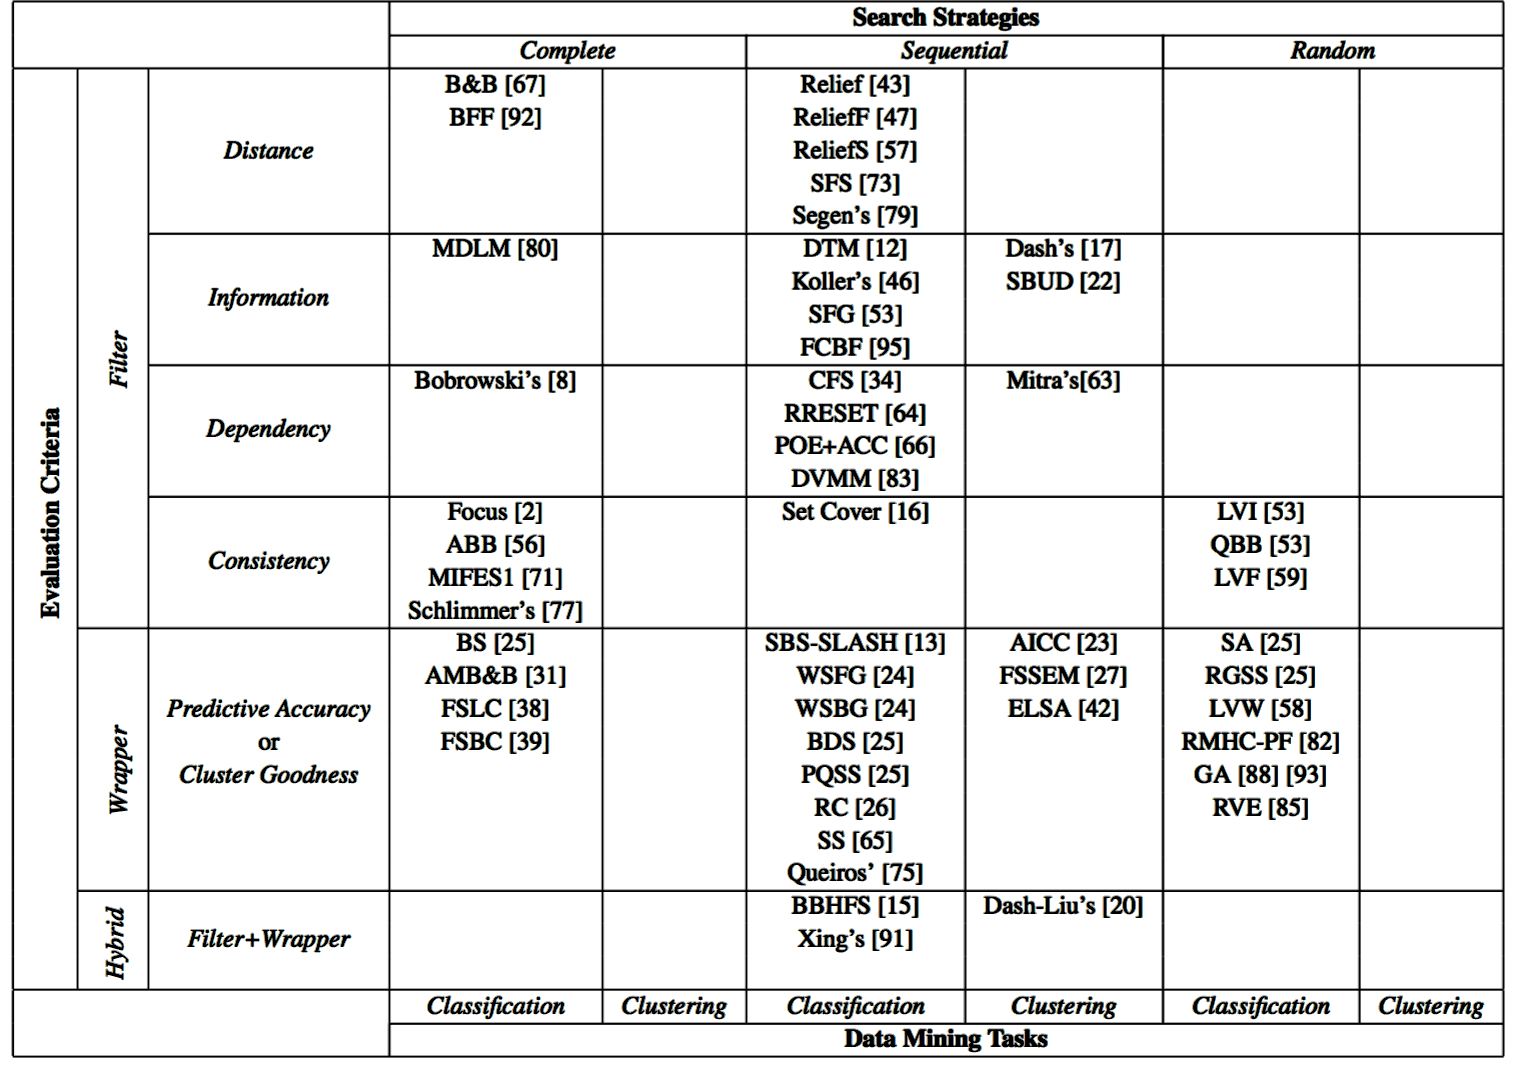
\includegraphics[scale=0.3]{img/img2-categorization-3d}
	\caption{Categorization of feature selection algorithms (Source: \cite{Liu:2005})} \label{fig:img2}
\end{figure}

Feature selection algorithms are categorized in three-dimensional framework in \cite{Liu:2005}. The three dimensions are evaluation criteria, search strategies and data mining tasks on which algorithms are more suitable to perform. We based our algorithms list on the categorization in Figure \ref{fig:img2} and added more up-to-date algorithms to the list.


%Beam search: complete search. sequential search adding (or removing) $p$ features in one step and removing (or adding) $q$ features in the next step $(p>q)$.

\subsection{Filter Methods}\label{ch2:alg:fil}

\begin{itemize}

\item Branch and Bound algorithm (B\&B) 
\newline B\&B \cite{Narendra:1977} is a search algorithm proposed in 1977. It is a depth-first-search tree-based feature elimination strategy, by evaluating the criterion at each level and sort them, continued with pruning. The advantage of this algorithm is: it guarantees that the selected subset yields the globally best value of any criterion that satisfies monotonicity. However, as it performs the full complete search, the number of subsets evaluated can be huge as the number of features grow. The complexity of the algorithm could grow to exponential.

\item Best First strategy for feature selection (BFF)
\newline BFF \cite{Xu:1988} was proposed as an improvement of B\&B algorithm. It is a heuristic search strategy that guarantee the globally best subset without exhaustive enumeration for any criterion that satisfies monotonicity. The advantage is that the number of subsets evaluated by BFF is less than those needed by B\&B algorithm. However, the complexity of the algorithm remains to be exponential as it utilizes  graph and compute the path to select subsets.

\item Relief
\newline Relief algorithm selects relevant features using a statistical method, does not depend on heuristics, is accurate even if features interact, and is noise-tolerant \cite{Kira:1992}. For each randomly selected instance, find nearest hit and miss to determine quality estimation. It can deal with nominal and numerical attributes, but it cannot deal with incomplete data and is limited to two-class problems. The complexity of this algorithm is $O(kN^2)$ (quadratic).

\item ReliefF
\newline ReliefF algorithm \cite{Kononenko:1994} is an variant of improvements of Relief algorithm. ReliefF tries to overcome Relief algorithm's limitation on handling only binary classes. ReliefF handles multiple classes and incomplete and noisy data. For each randomly selected instance, find nearest hit from the same class. For neighbours that are not in the same class, compute the miss. Update quality estimation for each attribute based on those difference. The complexity of the algorithm is improved to $O(kN)$, however, the optimal results are not guaranteed.

\item RReliefF
\newline ReliefF was further extended to RReliefF in order to handle continuous classes in regression. \cite{Robnik-Sikonja:1997} shows that RReliefF is effective in selecting features in learning regression trees for regression problems.

\item Relief with selective sampling (ReliefS)
\newline ReliefS was proposed on 2004 \cite{Liu:2004} as the improvement of Relief algorithm, which creates $kd$-tree upon each bucket of features and adds random sampling. The algorithm in Figure \ref{fig:img5} shows that ReliefS used either sample size $m$ or bucket size $t$ to control the $kd$-tree splitting process. With $N$ number of instances, $t = N/m$. Therefore, if $m$ is predetermined, the splitting process stops when it reaches the level where each bucket contains $N/m$ or fewer instances.  \cite{Liu:2004} also shows that ReliefS in general achieves better performance than ReliefF in terms of learning accuracy and hence selective sampling is an effective approach for active feature selection.

\begin{figure}
	\centering
	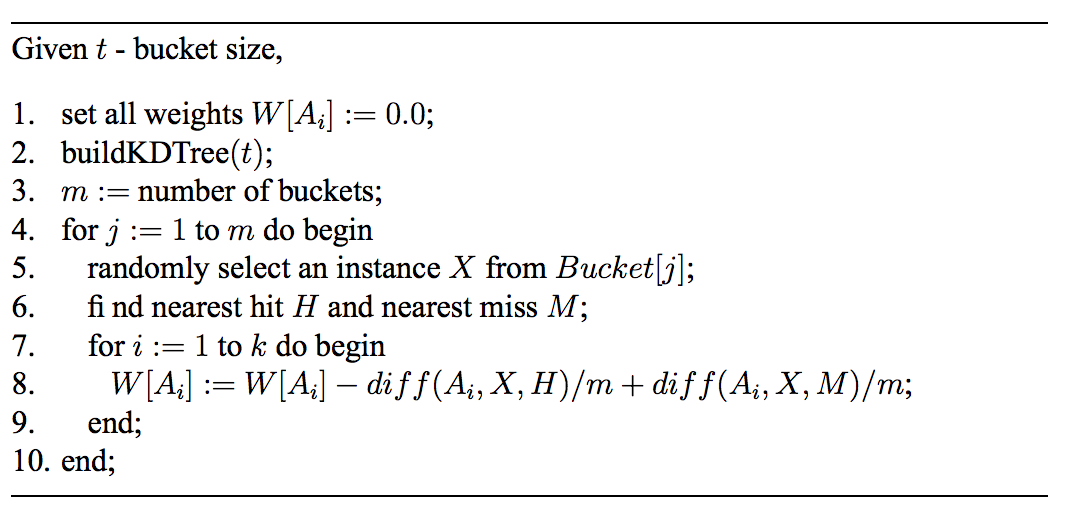
\includegraphics[scale=0.80]{img/img5-reliefs-pseudocode}
	\caption{Relief with selective sampling algorithm} \label{fig:img5}
\end{figure}

\item Sequential Feature Selection (SFS)
\newline Adds one feature which gives the highest value for the objective function, then the remaining features are added individually to the current subset and the new subset is evaluated. The individual feature is permanently included in the subset if it gives the maximum classification accuracy. The process is repeated until the required number of features are added. This is a naive SFS algorithm since the dependency between the features is not accounted for. The complexity of this algorithm is quadratic.

\item Sequential Floating Feature Selection (SFFS)
\newline This algorithm was proposed as an improvement of SFS algorithm. This algorithm works similarly to SFS but in addition, it adds another step which excludes one feature at a time from the subset obtained in the first step and evaluates the new subsets. The complexity of the algorithm remains to be quadratic.

\item Sequential Backward Selection (SBS)
\newline This algorithm works the same way as SFS algorithm, but it starts from a full set and removes a feature on each step. The process is repeated until the required number of features needed is achieved. The complexity of this algorithm is quadratic.

\end{itemize}


\subsection{Wrapper Methods}\label{ch2:alg:wra}

Wrapper methods are broadly classified into sequential selection algorithms and heuristic search algorithms \cite{Chandrashekar:2014}.

\begin{itemize}
\item Particle Swarm Optimization (PSO)
\newline This algorithm yields local optimum results are employed which can produce good results and are computationally feasible.
\item Genetic Algorithm (GA)
\newline This algorithm \cite{Yang:1998} also yields local optimum results are employed which can produce good results and are computationally feasible.
\end{itemize}

%The sequential selection algorithms start with an empty set (full set) and add features (remove features) until the maximum objective function is obtained. To speed up the selection, a criteria is chosen which incrementally increases the objective function until the maximum is reached with the minimum number of features. The heuristic search algorithms evaluate different subsets to optimize the objective function. Different subsets are generated either by searching around in a search- space or by generating solutions to the optimization problem. First we will look at sequential selection algorithms followed by the heuristic search algorithms.

\subsection{Embedded Methods}\label{ch2:alg:emb}

\begin{itemize}
\item Boosting Based Hybrid Feature Selection (BBHFS)
%\newline A major problem of forward selection methods is that it is difficult for them to select sets of features that are good copredictors of the class if none of these predictors is a good predictor of the class by itself.
\end{itemize}

\section{Parallel Algorithms}\label{ch2:par}


\section{Selected Algorithm}\label{ch2:sel}
